%!TEX root = paper.tex

\subsection{Combinatoric Names}
\label{sec:usecase-combinatoric}


\subsubsection{Gperftools packaging}

The gperftools tool from Google has gained popularity among some developers for
its high-performance thread-safe heap and its lite-weight profilers.  
Unfortunately, two issues made it difficult to maintain gperftools installations 
at LLNL.  First, gperftools is a C++ library.  Since C++ does not have standard 
ABI it needs to be re-built with each compiler and compiler version.  Second, 
building gperftools on atypical architectures (such as Blue Gene/Q) requires 
patches and a complicated configure lines that change with each compiler.  The 
first issue motivated application developers to try and maintain their own builds 
of gperftools that worked with their prefered compilers--a task that was made 
difficult by the second issue.

Spack presented a solution to both problems.  Package administrators can use Spack to 
easily maintain a central install of gperftools across the combinations of versions 
and compilers.  Spack's gperftools package also serves as a central repository for 
the knowledge of how to build gperftools on each platform and compiler combination.  

\begin{figure}
  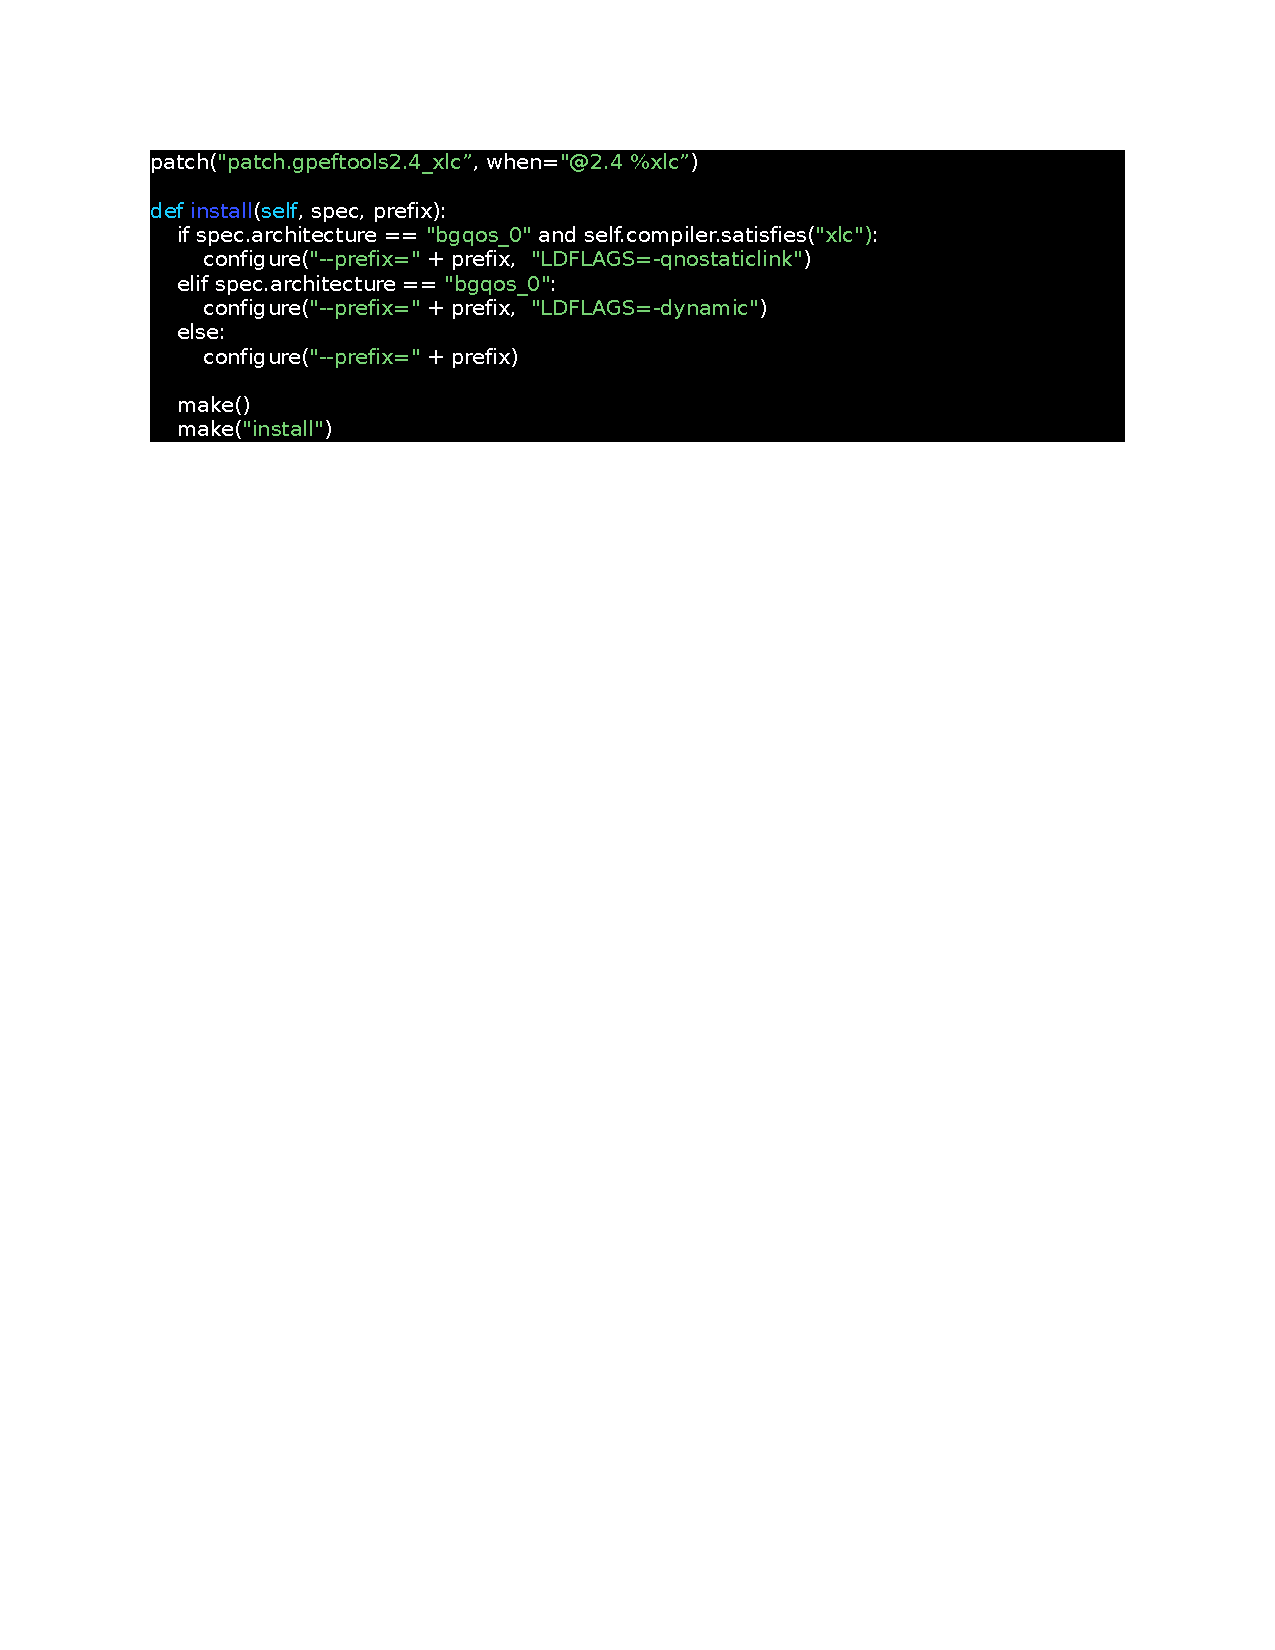
\includegraphics[width=\columnwidth]{code/gperftools.pdf}
  \caption{
    Simplified install routine for the gperftools tool.
    \label{fig:gperftools}
  }
\end{figure}

Figure~\ref{fig:gperftools} illustrates per-compiler and platform build rules with 
a simplified version of the install routine for the gperftools tool (Spack's real 
install routine for gperftools includes other compilers and more options per
compiler).  It applies a patch if gperftools 2.4 is built with the XLC compiler, 
and it selects the correct configure line based on the current platform and compiler.  

\subsubsection{{\tt mpileaks} packaging}
\todo{.5 page}
\begin{verbatim}
	- compiler x version x MPI x mpi version
\end{verbatim}

